%!TEX root = main.tex
\color{black}
\section{Evaluation and Results}\label{sec:eval_results}

In this section we aim at doing a comparative analysis on three different scenarios $\mathcal{S}_{\strict}$, $\mathcal{S}_{\loose}$ and $\mathcal{S}_{\real}$, built on top of the previously defined metrics. This comparison is done using standard cross-validation methodologies and a proposed temporal-based methodology.

We further provide an analysis on how to reduce the size of the training set, without compromising the final results.

\subsection{Evaluation}

With regards to our evaluation methodology, as we have previously mentioned, our purpose is to understand how laboratory conditions compare to real-world conditions.
We now detail how we achieve and compare these conditions.

Given the purpose of our work, we choose to measure our results by plotting an \gls{auroc} graph, which measures the \tpr~at different \fpr~levels, metrics that are commonly used across similar work~\cite{miller:rev_int,nissim:al_pdf,schultz:data_mining}.

The three scenarios that we will focus on will rely on metrics $\Mrealv$, $\Mloosev$ and $\Mstrictv$, over the dataset $\DD$:

\begin{itemize}
	\item Real Scenario $\mathcal{S}_{\real}$, applies the metric $\Mrealv$, containing 98,582 malware samples and 56,475 goodware samples.
	\item Loose Scenario $\mathcal{S}_{\loose}$, applies the metric $\Mloosev$, containing 45,306 malware samples and 1,989 goodware samples.
	\item Strict Scenario $\mathcal{S}_{\strict}$, applies the metric $\Mstrictv$, containing 24,658 malware samples and 1,989 goodware samples.
\end{itemize}

Given these three scenarios, we consider the following evaluation metrics:

\paragraph{Cross-validation (Figure \ref{fig:dia_xvalidation})}
To gain insight on how each model generalizes our scenarios, we apply a k-fold cross-validation, with $k=10$. This methodology splits the dataset into $k$ subsets (\ie, folds), selecting a single fold for validation and the remaining $k-1$ folds for training. This process is repeated $k$ times, ensuring every fold is used for validation and training.

\begin{figure}[!h]
	\centering
	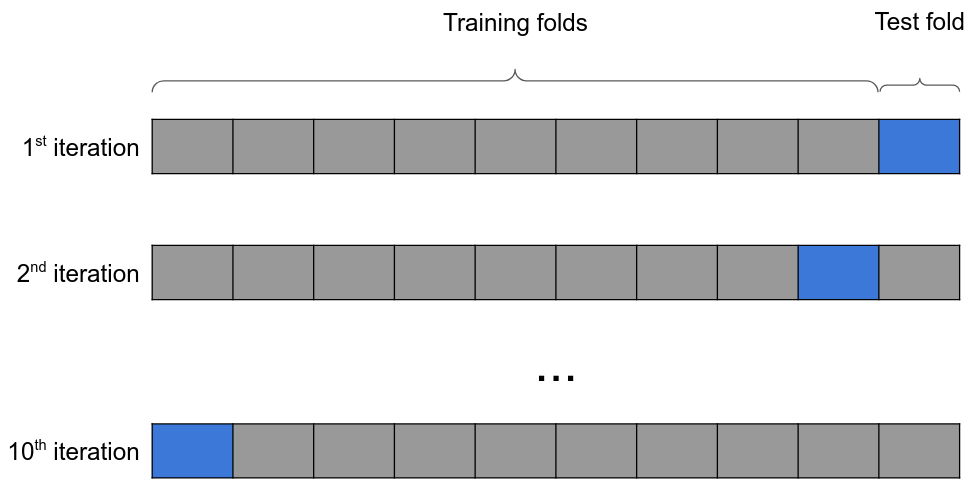
\includegraphics[width=\columnwidth]{dia_xvalidation}
	\caption{Cross-Validation evaluation example with 10 folds.}
	\label{fig:dia_xvalidation}
\end{figure}

Although the cross-validation methodology enables to measure the generalization capabilities of a model, it does not account for temporal ordering of the samples. Since we want to measure the score when training samples pre-date the validation samples, we now define a couple of temporal based validations. These are validated on the best performing model from cross-validation for all 3 scenarios.

\paragraph{Temporal based validation}
The first temporal based validation, which we designate as \textit{Past-to-Present validation}, Figure~\ref{fig:dia_pastpresent}, can be resumed as an iterative methodology where the validation set is fixed with the most recent samples, and the training set with the oldest. At each iteration the training set is extended with more recent samples and scored against the validation, until all samples are used.

\begin{figure}[!h]
	\centering
	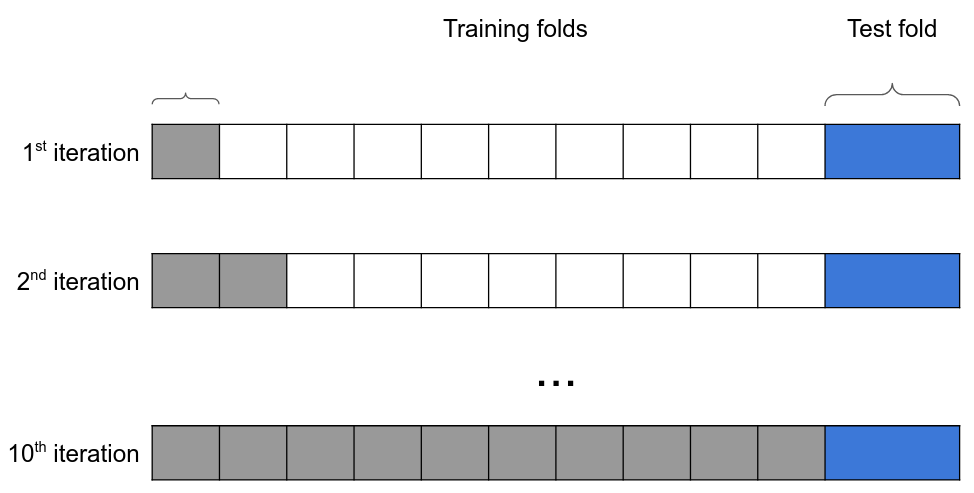
\includegraphics[width=\columnwidth]{dia_pastpresent}
	\caption{Past-to-Present evaluation example with 20/80 test/training, 10 folds in training.}
	\label{fig:dia_pastpresent}
\end{figure}


The second temporal based validation, which we designate as \textit{Present-to-Past validation}, Figure~\ref{fig:dia_presentpast}, is the opposite of \textit{Past-to-Present} with regards to the starting position of the training set. Again the validation is fixed the most recent samples, but now the training set starts with the temporally closest samples to the validation set. At each iteration the training set is extended, this time with older samples and scored against the validation, until all samples are used.

\begin{figure}[!h]
	\centering
	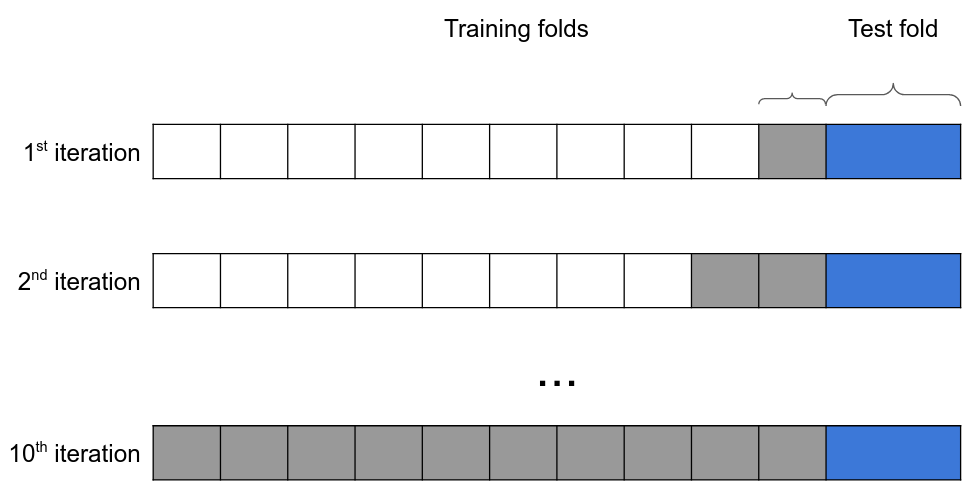
\includegraphics[width=\columnwidth]{dia_presentpast}
	\caption{Present-to-Past evaluation example with 20/80 test/training, 10 folds in training.}
	\label{fig:dia_presentpast}
\end{figure}

\textit{Past-to-Present} and \textit{Present-to-Past} validations both require two parameters, specifically the size of the validation set, and how the increments to the training set are made. For our evaluation, we use the 20\% most recent samples as validation, and split the remaining 80\% into 10 folds, hence the validation is done 10 times, with each iteration increasing the training size by one fold.

These two validation methodologies give us the ability to account for temporal consistency. Moreover, they enable us to compare the importance of older \textit{vs} newer samples to classify recent samples.

We designate the third and last temporal based validation as \textit{Temporal Window validation}, Figure~\ref{fig:dia_slidingwindow}. This validation methodology is inspired on regular cross-validation, in the sense that it splits the dataset into folds, but changes how the folds are used. Specifically it takes $n$  temporal consistent and contiguous folds, \ie, each fold immediately precedes the next one, and uses the last fold (more recent samples) for validation, and the previous folds for training (older samples). By starting with the $n$ first folds and sliding one fold on each iteration, we apply a sliding window of size $n$ over the dataset.

\begin{figure}[!h]
	\centering
	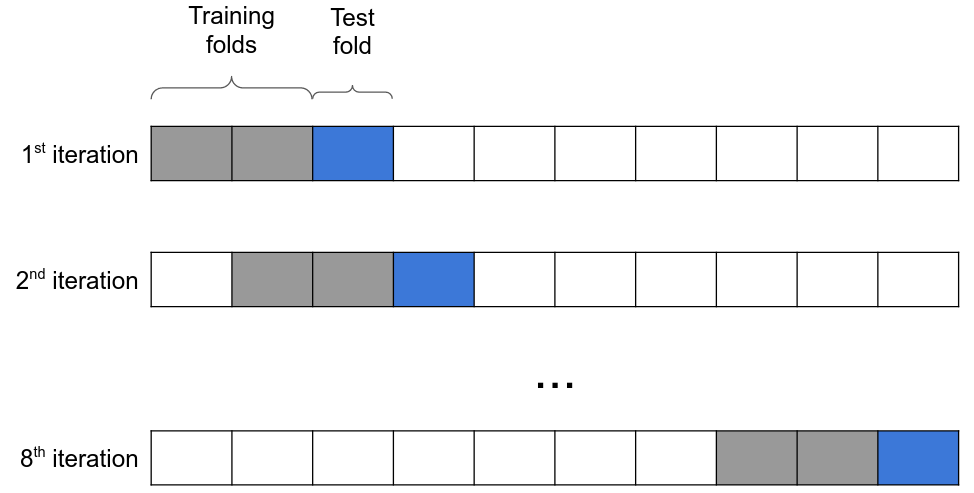
\includegraphics[width=\columnwidth]{dia_slidingwindow}
	\caption{Temporal window evaluation example with window of size 3 over a 10 fold dataset.}
	\label{fig:dia_slidingwindow}
\end{figure}

For this last validation methodology, we again split the dataset into 10 folds. The sliding window size, $n$, is chosen during the results phase, as its choice depends on previous results.

We measure the \gls{auroc} during each validation's iteration and use the average measurement to discuss the results.

\subsection{Results}
\label{section:single_layer_results}

We implement our experiments in Python, by using Jupyter Interactive Notebooks\cite{tool:jupyter} to facilitate data visualization. We use scikit-learn\cite{tool:sklearn} for \gls{ml}, and Pandas\cite{tool:pandas} for data analysis. Our experiments were conducted on an Ubuntu Virtual Machine with 16 cores and 16GB of RAM, in order to minimize training and validation times.

We now focus on applying the evaluation methodologies to our scenarios. This enables us to compare the different conditions, and consequently results, that affect malware detection.

%We compare each model $\mathcal{LR}$ and $\mathcal{E}$ under each scenario $\mathcal{S}_{\strict}$, $\mathcal{S}_{\loose}$ and $\mathcal{S}_{\real}$.

We start with what we determine as \textit{laboratory conditions}, ideal conditions for the problem of malware detection. These are met when we apply the strict metrics $\Mstrictv$, to the dataset $\mathcal{C}$, obtaining scenario $\mathcal{S}_{\strict}$.

Under these conditions, our model provides the best results, with an \gls{auroc} of 0.91, as shown by the red curve in Figure \ref{fig:xval_results}. We argue that such high values are easily attained from factors like a small and reliable dataset, and the use of cross-validation, which mixes samples and ignores possible dependencies on malware samples.

\begin{figure}[!h]
	\centering
	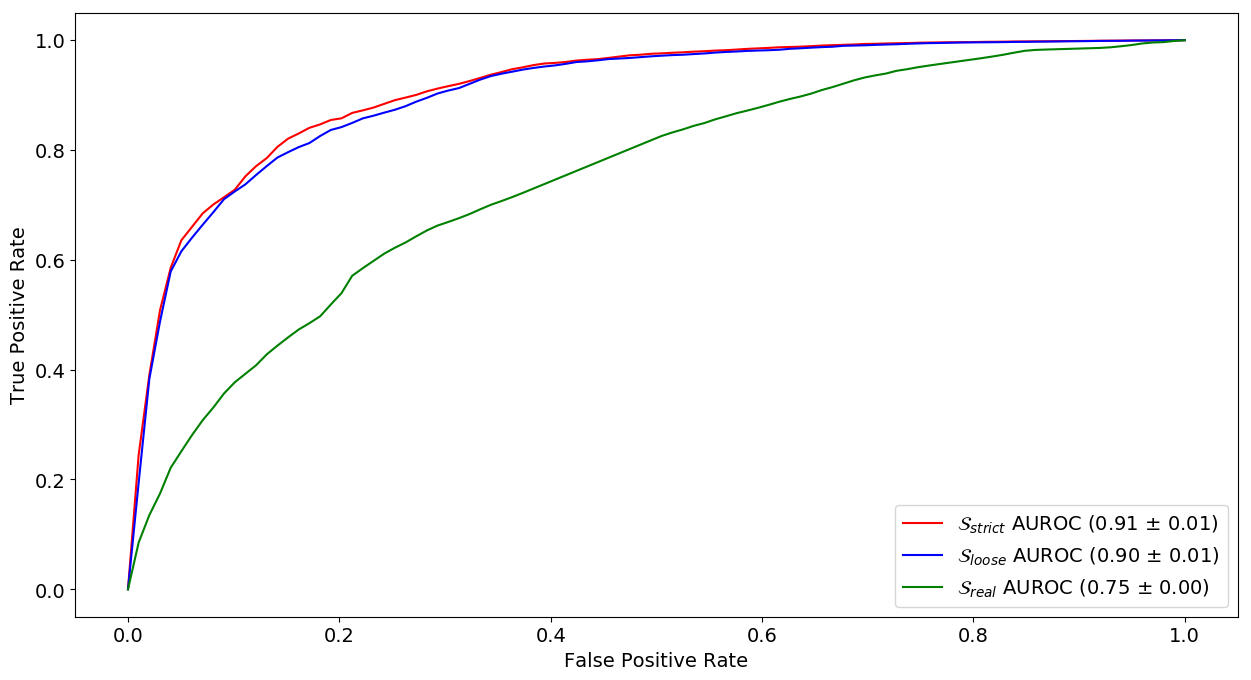
\includegraphics[width=\columnwidth]{xval_results}
	\caption{Cross-Validation \gls{roc} and \gls{auroc} for our model under $\mathcal{S}_{\strict}$, $\mathcal{S}_{\loose}$ and $\mathcal{S}_{\real}$.}
	\label{fig:xval_results}
\end{figure}

To understand how reliability influences the models' result, we use scenarios $\mathcal{S}_{\loose}$ and $\mathcal{S}_{\real}$, which are less reliable and include more samples.

Under these more relaxed, \textit{real-world} conditions, the model's results hold an \gls{auroc} of 0.90 under $\mathcal{S}_{\loose}$, as shown by the blue curve in Figure \ref{fig:xval_results}, and an \gls{auroc} of 0.75 under $\mathcal{S}_{\real}$, as seen by the green curve in Figure \ref{fig:xval_results}.

From $\mathcal{S}_{\strict}$ to $\mathcal{S}_{\loose}$, the only change is the amount of malware labeled samples, which significantly increase.
The difference is interesting, as although the number of malware labeled samples increase significantly, the results are not that affected.
This suggests that although the reliability for malware decreases, its impact is not as noticeable as expected.
This might also suggest that vendors do converge on their definition of malware, under our $\Mloosev$ metric.
If vendors did not converge on what is malware, adding more samples would culminate in worse results, as separation between malware and goodware would become harder.

When looking at the changes from $\mathcal{S}_{\loose}$ to $\mathcal{S}_{\real}$, not only the amount of malware labeled samples increase, but also the number of goodware labeled samples, both by a significant amount. 
The way this impacts the results is pretty significant, as we observe a high decrease in the \gls{auroc}.
The metric $\Mrealv$ that labels malware and goodware for this scenario $\mathcal{S}_{\real}$ disregards the cross-check from outside repositories, which in turn degrade the reliability significantly, as well as increase the dataset size notably.
We attribute the results' degradation mainly to the unreliability of goodware labeling, not only because we have previously seen that increase in malware does not significantly impact results (from $\mathcal{S}_{\strict}$ to $\mathcal{S}_{\loose}$), but also due to the tendency for false negatives in vendors (Figure \ref{fig:distribution_changes}), which in turn lead us to incorrectly label goodware for the samples in $\mathcal{C}$.

The results we described show how moving from \textit{laboratory conditions} to more \textit{real-world conditions} degrade the model's performance. We now focus on using our previously defined temporal based methodologies to further converge into a real-world scenario.

\medskip

We start by applying our \textit{Past-to-Present} validation to the three scenarios, $\mathcal{S}_{\strict}$, $\mathcal{S}_{\loose}$ and $\mathcal{S}_{\real}$.
As previously defined, this validation starts with an older set of training samples and iteratively adds newer samples, validating each iteration on a fixed set of the most recent samples.
Since our interest is to measure performance variation over time, we plot in Figure~\ref{fig:pastpresent} the \gls{auroc} at every iteration (\ie, fold), for each of our three scenarios.

\begin{figure}[!h]
	\centering
	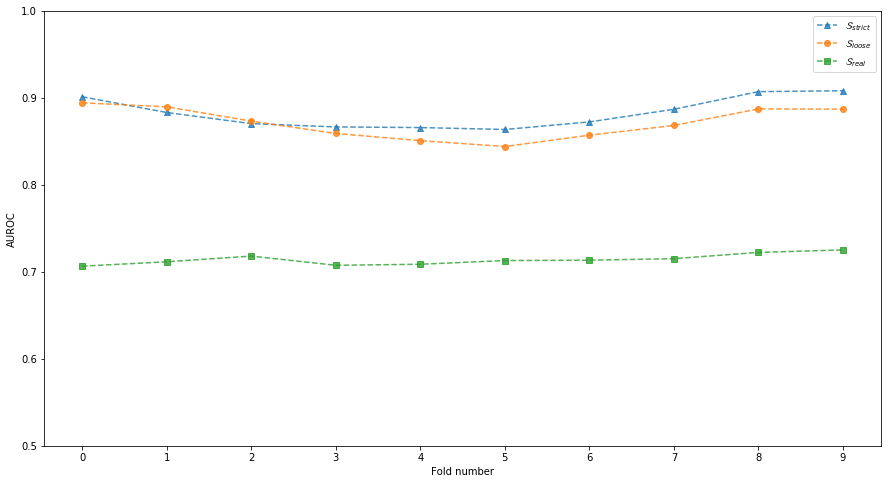
\includegraphics[width=\columnwidth]{pastpresent}
	\caption{\gls{auroc} for each iteration of the \textit{Past-to-Present} evaluation. Folds order consistent with temporal order (\ie, fold 0 contains older samples than fold 1)}
	\label{fig:pastpresent}
\end{figure}

When directly comparing the average \gls{auroc} for cross-validation and our \textit{Past-to-Present} validation, we note that for both $\mathcal{S}_{\strict}$ and $\mathcal{S}_{\loose}$ the \gls{auroc} remains identical, while for $\mathcal{S}_{\real}$ the score decreases from 0.75 to 0.67.
This decrease is intuitive to the methodology, as we are forcing temporal consistency between samples.

For both $\mathcal{S}_{\strict}$ and $\mathcal{S}_{\loose}$ we note only a slight increase as new folds are added.
They still relate, as we have previously noted for cross-validation, arguably given their metrics $\Mstrictv$ and $\Mloosev$ are not very different.
The small variation to the cross-validation methodology can be justified by using small dataset size for both cases.

As for $\mathcal{S}_{\real}$ we note higher variation and lower overall score, as the reliability of the metric $\Mrealv$ goes down.
This is expected, not only because we are enforcing temporal consistency between samples, but as new folds are added, the training gets bigger, while the test remains the same.

Our main observation for this validation methodology is that there is a slight tendency for \gls{auroc} to increase, as we move forward in time, close to the validation set.

From these observations, we argue about the possibility that with fixed validation set of the most recent samples, a model benefits by using samples temporally closer to validation.

\medskip

Our next result, which uses our \textit{Present-to-Past} validation methodology will further help analyze the aforementioned detail.
The \textit{Present-to-Past} validation enhances the previous results under real-world conditions. 
This methodology starts by fixing the validation set to the most recent samples, but with the training set starting at the temporally closest samples to validation.
At each iteration, older samples are added to the training set and validated on the fixed, most recent, samples.

By applying this methodology to the three scenarios, $\mathcal{S}_{\strict}$, $\mathcal{S}_{\loose}$ and $\mathcal{S}_{\real}$, we plot Figure \ref{fig:presentpast}, where the X axis increases as older samples are added to the training set (\eg\ fold 0 contains newer samples than fold 1), hence measuring the performance variance over time. Similarly to the previous observation, the average \gls{auroc} suffers a decrease when compared to cross-validation.
For $\mathcal{S}_{\strict}$ we note a change from 0.91 to 0.90, for $\mathcal{S}_{\loose}$ the score is the same, and for $\mathcal{S}_{\real}$ 0.75 to 0.69.

\begin{figure}[!h]
	\centering
	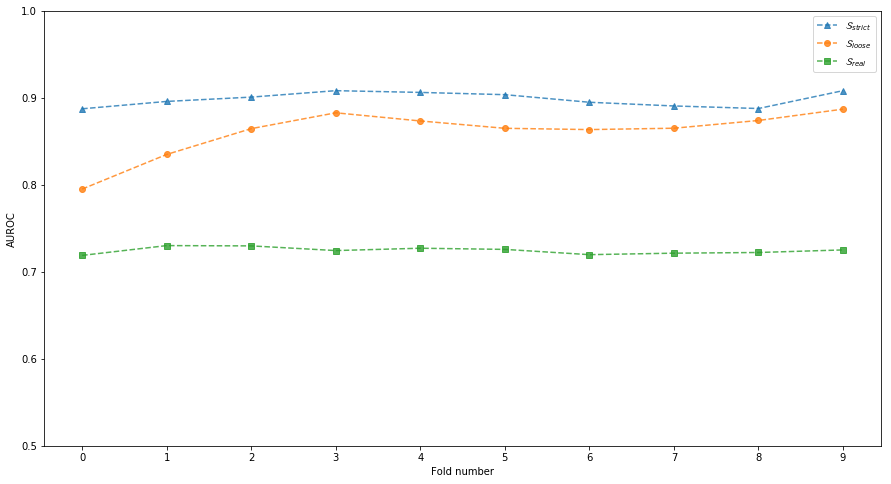
\includegraphics[width=\columnwidth]{presentpast}
	\caption{\gls{auroc} for each iteration of the \textit{Present-to-Past} evaluation. Folds order is the inverse of temporal order (\ie, fold 0 contains newer samples than fold 1)}
	\label{fig:presentpast}
\end{figure}

The comparison between scenarios is identical to what was observed in cross-validation and \textit{Past-to-Present}: scenarios $\mathcal{S}_{\strict}$ and $\mathcal{S}_{\loose}$ display very similar results, with $\mathcal{S}_{\real}$ dropping behind due to its less reliable labeling metric.
It is noticeable that using the entire dataset does not bring much improvement to the final results. In fact, for $\mathcal{S}_{\real}$ the score even drops after fold $\#2$.

With these results, our original observation that samples closer to the validation set benefit the model becomes more convincing. In fact, we argue that there should be an ideal number of necessary training folds, temporally consistent with the validation fold (\ie\ any fold from training predates validation), needed to maximize the overall score.

\medskip

Finally, we analyze how does such reduced training set behaves in our scenarios; for this purpose, we define a sliding window that moves forward in time through each scenario for training and validation.
We propose a reduction on the training size to $n=3$ folds predating the validation fold.
We choose $n = 3$, since we have seen that the scores either do not improve (for $\mathcal{S}_{\strict}$ and $\mathcal{S}_{\loose}$) or actually go down (for $\mathcal{S}_{\real}$) with higher folds.
In summary, we have selected 30\% of each dataset for training purposes and the next 10\% for validation (3 training folds, 1 validation fold), and then started moving the window forward in time (1 fold at a time) to obtain the following results (Figure~\ref{fig:slidingwindow}): for  $\mathcal{S}_{\strict}$, $\mathcal{S}_{\loose}$ and $\mathcal{S}_{\real}$, we obtain \gls{auroc} values of 0.89, 0.88 and 0.76, respectively. 
These results come to reaffirm our argument that we can reduce the size of the training set, without losing any significant score.

\begin{figure}[!h]
	\centering
	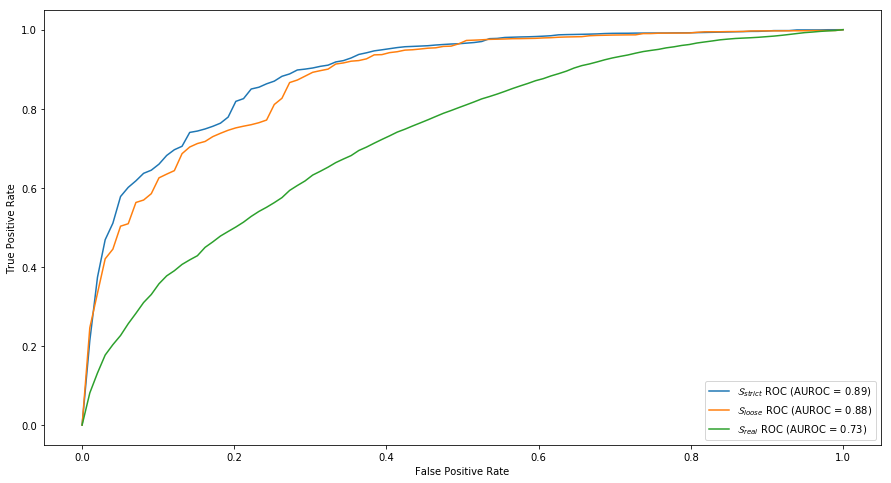
\includegraphics[width=\columnwidth]{slidingwindow}
	\caption{\gls{roc} and \gls{auroc} for our three scenarios, under the \textit{Temporal Window} methodology.}
	\label{fig:slidingwindow}
\end{figure}

Comparing these results with the baseline cross-validation, we note a decrease for each scenario, specifically a decrease from 0.91 to 0.89 for $\mathcal{S}_{\strict}$, from 0.90 to 0.88 for $\mathcal{S}_{\loose}$ and from 0.75 to 0.73 for $\mathcal{S}_{\real}$.
We should highlight that the results that use temporal consistency should better reflect the reality than standard cross-validation, since we are requiring temporally ordered samples.
Another important idea that should be stressed is that for cross validation we used a fairly reasonable amount of data for training purposes, whereas in this last case we used a restricted amount of data. This might be a relevant issue in a few year's time. The results obtained are summarized in Table \ref{tab:singlelayer_results}.

\begin{table}[!htb]
	\renewcommand{\arraystretch}{1.2} % more space between rows
	\centering
	\begin{tabular}{l|cccc}
		AUROC & $\DS_\strict$ & $\DS_\loose$ & $\DS_\real$ & Train/Test \%\\
		\hline
		Cross-Validation & 0.91 & 0.90 & 0.75 & 90 / 10\\
		Past-to-Present & 0.90 & 0.90 & 0.67 & 10 to 90 / 10\\
		Present-to-Past & 0.90 & 0.90 & 0.69 & 10 to 90 / 10\\
		Sliding-Window & 0.89 & 0.88 & 0.73 & 30 / 10\\
		\hline
	\end{tabular}
	\smallskip
	\caption{Single layer results summary.}
	\label{tab:singlelayer_results}
\end{table}

\medskip

With a better understanding of how the model behaves under different methodologies, we now diverge to how we improved not only the overall results, but also the information provided by the model.
